\documentclass[11pt,a4paper]{article}

% ── Idioma y codificación ──
\usepackage[spanish,es-nodecimaldot]{babel}
\usepackage[utf8]{inputenc}
\usepackage[T1]{fontenc}

% ── Tipografía ──
\usepackage{lmodern}
\usepackage{microtype}

% ── Matemáticas ──
\usepackage{amsmath,amssymb,mathtools,bm}

% ── Tablas y figuras ──
\usepackage{booktabs,multirow}
\usepackage{graphicx}
\usepackage{subcaption}
\usepackage{float}

% ── Código y colores ──
\usepackage{xcolor}
\usepackage{listings}

% ── Layout ──
\usepackage[margin=2.5cm]{geometry}
\usepackage{setspace}
\onehalfspacing

% ── Referencias ──
\usepackage[numbers,sort&compress]{natbib}
\usepackage[colorlinks=true,linkcolor=blue!60!black,citecolor=green!50!black,urlcolor=blue!70!black]{hyperref}

% ── Macros ──
\newcommand{\zb}{z_b}
\newcommand{\pd}[2]{\frac{\partial #1}{\partial #2}}
\newcommand{\RMSE}{\mathrm{RMSE}}
\newcommand{\NRMSE}{\mathrm{NRMSE}}
\DeclareMathOperator{\relu}{ReLU}
\DeclareMathOperator{\softplus}{softplus}
\newcommand{\pendiente}[1]{\textit{[Pendiente: #1]}}

% ── Metadata ──
\title{Inversión de Batimetría mediante Redes Neuronales Informadas por Física:\\
       Revisión de Literatura y Resultados Experimentales}
\author{Etienne Calderon}
\date{\today}

% ============================================================
\begin{document}
\maketitle

\begin{abstract}
Este reporte resume el estado del arte en inversión de batimetría
basada en las ecuaciones de aguas someras (SWE) mediante redes neuronales
informadas por física (PINNs), y presenta los resultados experimentales
obtenidos hasta la fecha. Se comparan arquitecturas, formulaciones de ecuaciones
y estrategias de regularización de cinco trabajos clave, y se validan
las decisiones de diseño del enfoque propuesto con experimentos sintéticos.
Un experimento con datos reales de laboratorio (Angel et al.) revela una
limitación estructural de la inversión PINN de penalización blanda frente
a métodos de restricción dura, documentada como hallazgo y trabajo futuro.
\end{abstract}

\tableofcontents
\newpage

% ── Secciones ──
\section{Introducción}
\label{sec:intro}

% P1 — Definición + fuente
La batimetría es la medición y representación de la profundidad y el relieve
del fondo de un cuerpo de agua respecto de un nivel de referencia vertical, y
constituye en esencia el equivalente sumergido de la topografía terrestre
\cite{wolfl2019, talley2011}. Describe tanto la profundidad local como la
forma del lecho de océanos, estuarios, ríos y lagos.

% P2 — Por qué importa
La batimetría es un insumo fundamental de la hidráulica, la hidrología y las
ciencias costeras y oceánicas. El lecho impone la condición de borde inferior
sobre la que se desarrolla todo el flujo, de modo que la propagación de
inundaciones y tsunamis, la circulación de mareas y corrientes, el transporte
de sedimentos y la seguridad de la navegación dependen de ella. En la práctica,
la fidelidad de cualquier modelo hidrodinámico está acotada por la fidelidad de
la batimetría que se le suministra.

% P3 — Cómo funciona el sonar multihaz
El levantamiento batimétrico directo se realiza principalmente mediante dos
tecnologías. La primera es la ecosonda multihaz, instalada en una embarcación,
que emite un abanico de haces acústicos transversales a la trayectoria y mide
el tiempo de viaje de ida y vuelta de cada eco reflejado por el fondo. Conocida
la velocidad del sonido en la columna de agua, ese tiempo y el ángulo del haz
determinan la profundidad y la posición de cada sondaje sobre una franja ancha,
que se cubre de forma continua a medida que la embarcación avanza
\cite{lurton2010}.

% P4 — Cómo funciona el LiDAR batimétrico
La segunda es el LiDAR batimétrico aerotransportado, que emite pulsos de láser
de longitud de onda verde capaces de penetrar la columna de agua. La
profundidad se obtiene de la diferencia temporal entre el retorno reflejado por
la superficie libre y el reflejado por el fondo, lo que permite cartografiar con
rapidez aguas someras y claras desde una aeronave \cite{guenther2000,
szafarczyk2023}.

% P5 — Brecha de cobertura / costo (citada, redacción conservadora)
Ambas técnicas son precisas pero lentas, costosas y logísticamente limitadas:
requieren plataformas dedicadas, condiciones operativas favorables y campañas
que deben repetirse, porque el lecho evoluciona por sedimentación y erosión.
Como resultado, solo una fracción del fondo oceánico mundial está cartografiada
con métodos acústicos modernos, del orden de una cuarta parte a mediados de la
década de 2020 frente a apenas unos pocos puntos porcentuales una década antes,
y la cobertura por sonar multihaz de alta resolución es considerablemente menor
\cite{wolfl2019}. Esta brecha persistente motiva el desarrollo de métodos
indirectos que infieran el fondo a partir de observaciones más accesibles.

% P6 — Genérico, sin nombrar Chile
%% IEEE-CUT: en la versión IEEE este párrafo se reduce a media frase ("regiones costeras con datos escasos").
El déficit es más severo donde los levantamientos son escasos, gruesos o están
desactualizados: incluso un sitio ya sondeado pierde vigencia porque el lecho
evoluciona por sedimentación y erosión, de modo que la necesidad no es solo
cartografiar por primera vez, sino actualizar batimetría obsoleta o de baja
resolución, a menudo en tramos de difícil acceso. Frente a ese costo, el
monitoreo del nivel del agua es barato, continuo y permanente, y no requiere un
levantamiento batimétrico para operar: los registros de nivel mareal y de nivel
y caudal fluvial se acumulan de forma sostenida justo allí donde falta una
batimetría distribuida de alta resolución. Las mediciones de velocidad
superficial aportan una restricción más fuerte, pero son más escasas y suelen
asociarse a despliegues dedicados; aun así pueden obtenerse de forma
independiente, por ejemplo mediante boyas a la deriva, velocimetría por video o
radar de alta frecuencia, por lo que el valor central del enfoque descansa sobre
la señal de nivel y su variación temporal. Surge así la oportunidad de un método
inverso que actualice batimetría obsoleta o gruesa, incluso en tramos
inaccesibles, a partir de datos de superficie que ya se registran de forma
continua, en lugar de encargar nuevas campañas.

% P7 — Idea del problema inverso (lenguaje natural, sin notación)
La idea central de este trabajo es, en lugar de medir el fondo directamente,
inferirlo de la huella que deja sobre el agua. La forma del lecho controla cómo
se elevan y deforman la superficie libre y cómo se aceleran las corrientes; por
lo tanto, las observaciones de la superficie y del flujo contienen información
sobre el fondo no observado. Recuperar el lecho a partir de esas observaciones
es un problema inverso, mal planteado en general, que se vuelve tratable cuando
se lo restringe con la física que gobierna el agua somera.

% P8 — El enfoque (conceptual; notación diferida)
Para resolver ese problema inverso, esta tesis adopta las \textbf{redes
neuronales informadas por física} (PINNs) \cite{raissi2019}: redes entrenadas
para ser consistentes, de forma simultánea, con las observaciones de superficie
y con las ecuaciones de aguas someras que gobiernan el flujo. Bajo esa doble
restricción, el fondo desconocido emerge como el campo que explica los datos y
satisface las ecuaciones a la vez. El enfoque emplea, conceptualmente, un
modelo para el campo de flujo y otro independiente para el lecho. La
formulación matemática de las ecuaciones de aguas someras y toda la notación se
introducen en la Sección~\ref{sec:problema}; la arquitectura y la
función de pérdida, en la Sección~\ref{sec:method}.

\section{Definición del Problema}
\label{sec:problema}

Se observa la superficie libre del agua y, cuando está disponible, el flujo, y
se desea recuperar la geometría del fondo que no se ha medido. Para que esa
recuperación sea posible se necesita un modelo físico que vincule lo observable
en la superficie con el fondo desconocido: las ecuaciones de aguas someras
(SWE). Esta sección deriva brevemente las SWE, enuncia las hipótesis bajo las
que son válidas, explica por qué su estructura permite la inversión, y fija la
notación empleada en el resto del documento.

\subsection{De Navier--Stokes a las ecuaciones de aguas someras}

El punto de partida son las ecuaciones de Navier--Stokes para un fluido
incompresible, es decir, la conservación de masa y de cantidad de movimiento
\cite{vreugdenhil1994, vallis2017}. Las SWE se obtienen integrándolas en la
vertical bajo las siguientes hipótesis:

\begin{enumerate}
  \item \textbf{Continuo e incompresibilidad.} El agua se trata como un medio
        continuo de densidad constante $\rho$.
  \item \textbf{Aguas someras (onda larga).} La escala vertical es mucho menor
        que la horizontal, $(H/L)^2 \ll 1$. La aceleración vertical es
        despreciable y la presión resulta hidrostática, $\pd{p}{z} = -\rho g$,
        de donde $p = \rho g\,(\eta - z)$.
  \item \textbf{Velocidad uniforme en la vertical.} El perfil vertical de
        velocidad se considera aproximadamente uniforme; todas las variables de
        las SWE son promedios en la profundidad.
  \item \textbf{Fondo impermeable y fijo.} No hay flujo a través del lecho y la
        batimetría no cambia en el tiempo, $\pd{\zb}{t} = 0$; en la superficie
        libre se impone la condición cinemática.
  \item \textbf{Cierre de fricción.} El esfuerzo de fondo se parametriza con la
        fórmula de Manning; la viscosidad molecular es despreciable frente a la
        turbulenta a números de Reynolds altos.
\end{enumerate}

Integrando la continuidad y la cantidad de movimiento entre el fondo
$\zb(x,y)$ y la superficie $\eta(x,y,t)$ mediante la regla de Leibniz, y
aplicando las condiciones de borde anteriores, se obtienen las SWE
bidimensionales en forma primitiva:

\begin{align}
  \pd{h}{t} + \pd{(hu)}{x} + \pd{(hv)}{y} &= 0,
    \label{eq:swe-cont}\\
  \pd{u}{t} + u\pd{u}{x} + v\pd{u}{y} &= -\,g\,\pd{(h+\zb)}{x} - S_{fx},
    \label{eq:swe-momx}\\
  \pd{v}{t} + u\pd{v}{x} + v\pd{v}{y} &= -\,g\,\pd{(h+\zb)}{y} - S_{fy},
    \label{eq:swe-momy}
\end{align}

donde $h$ es la profundidad, $(u,v)$ las velocidades promediadas en la
vertical, $\zb$ la batimetría y $S_{fx} = g\,n^2\,u\,\lVert\mathbf{u}\rVert /
h^{4/3}$ la pendiente de fricción de Manning (coeficiente $n$; análogo para
$S_{fy}$). La misma física admite formas equivalentes. En la forma
\emph{conservativa} las incógnitas son las cantidades conservadas
$(h, hu, hv)$ y las ecuaciones se escriben como la divergencia de unos flujos
más un término fuente que recoge la pendiente del fondo y la fricción; conserva
masa y momento de forma exacta, pero obliga a recuperar la velocidad como
$u = hu/h$, inestable cuando $h \to 0$ (zonas que se secan). La forma
\emph{primitiva-conservativa} multiplica el residuo primitivo por una matriz
que reescala automáticamente cada ecuación, uniendo la estabilidad de las
variables primitivas con la ponderación de la conservativa. La elección de la
forma del residuo empleada por el método se discute en la
Sección~\ref{sec:method}.

\subsection{Por qué la batimetría es recuperable}

El término de presión hidrostática introduce el acoplamiento
$-\,g\,\pd{(h+\zb)}{x} = -\,g\,\pd{\eta}{x}$, con $\eta = h + \zb$ la
elevación de la superficie libre. Ese término es el \emph{canal de información}
entre lo observable ($\eta$) y lo desconocido ($\zb$): una sola instantánea es
equifinal, pues infinitas particiones $(h,\zb)$ producen el mismo $\eta$, pero
la evolución temporal del flujo depende de $\zb$ a través de este acoplamiento,
lo que rompe la degeneración y vuelve tratable el problema inverso.

\subsection{Validez y límite de aplicabilidad}

Las SWE son válidas mientras $(H/L)^2 \ll 1$, equivalente a $k h \ll 1$ para
una perturbación de número de onda $k$: ondas largas, no dispersivas, que se
propagan a velocidad $c = \sqrt{g h}$ \cite{leveque2002, vallis2017}. Cuando
$k h$ se acerca a la unidad aparecen efectos dispersivos que las SWE no
capturan; este límite se manifiesta empíricamente en el Exp.~6
(Sección~\ref{sec:exp6}), con datos de canal de oleaje en régimen
$k h \approx 1.3$.

\subsection{Diferencias con Navier--Stokes}

Frente a las ecuaciones de Navier--Stokes tridimensionales, las SWE reducen el
problema de 3D a 2D; la hipótesis hidrostática elimina la ecuación vertical de
cantidad de movimiento; no se resuelve el perfil vertical de velocidad sino su
promedio; la turbulencia tridimensional no se resuelve, sino que se parametriza
mediante la fricción de fondo. El costo computacional es mucho menor, a cambio
de un dominio de validez acotado a flujos de aguas someras.

\subsection{Notación}

La Tabla~\ref{tab:notacion} resume la notación empleada en el resto del
documento.

\begin{table}[H]
\centering
\caption{Notación empleada en el documento.}
\label{tab:notacion}
\begin{tabular}{ll}
\toprule
Símbolo & Significado \\
\midrule
$x,\ y$              & Coordenadas horizontales \\
$t$                  & Tiempo \\
$h$                  & Profundidad del agua \\
$u,\ v$              & Velocidades promediadas en la vertical \\
$\zb$                & Batimetría (elevación del fondo), $\pd{\zb}{t}=0$ \\
$\eta = h + \zb$     & Elevación de la superficie libre \\
$g$                  & Aceleración de gravedad \\
$n$                  & Coeficiente de Manning \\
$q = h u$            & Caudal por unidad de ancho \\
$S_f$                & Pendiente de fricción \\
$Fr = u/\sqrt{g h}$  & Número de Froude \\
$c = \sqrt{g h}$     & Velocidad de onda larga \\
\bottomrule
\end{tabular}
\end{table}

\section{Revisión de Literatura}
\label{sec:lit}

Esta sección resume seis trabajos representativos sobre reconstrucción de
batimetría y modelado de aguas someras con redes neuronales y métodos de
optimización, ordenados por relevancia para esta tesis. Cada uno se describe con
la misma estructura: problema, entrada y salida, datos, método, resultados clave
y relación con esta tesis. La Tabla~\ref{tab:lit-overview} los resume de un
vistazo.

%% IEEE-CUT: en la versión IEEE cada artículo se comprime a 1--2 frases; los bloques \paragraph{} detallados son solo para la tesis.

\begin{table}[H]
\centering
\caption{Panorama de los trabajos revisados.}
\label{tab:lit-overview}
\begin{tabular}{@{}llll@{}}
\toprule
Trabajo & Problema & Entrada $\to$ Salida & Método \\
\midrule
Dazzi (2024) & Directo               & BC, IC $\to (h,u,\zb)$      & PINN, MLP único \\
Ohara (2024) & Inverso conjunto      & $u,\eta \to (h,u,v,\zb,n)$  & PINN, red por campo \\
Tian (2025)  & Directo (formas)      & dominio $\to (h,u,v)$       & PINN, FNN única \\
Chen (2023)  & Inverso (costero)     & oleaje $\to \zb$            & PINN, ec.\ de oleaje \\
Angel (2024) & Inverso, datos reales & $\eta$ de sensores $\to \zb$ & Adjunto-EDP \\
Liu (2024)   & Inverso, dos etapas   & $\eta \to \zb$              & Surrogado CNN \\
\bottomrule
\end{tabular}
\end{table}

% ──────────────────────────────────────────────────────────────
\subsection{Dazzi et al.\ (2024) --- PINNs con SWE aumentado}
\label{sec:lit:dazzi}

\paragraph{Problema.}
\cite{dazzi2024} resuelven el problema \emph{directo} de las SWE con un sistema
\emph{aumentado} que incorpora la batimetría como variable: a las ecuaciones de
masa y momento se añaden dos relaciones. La primera, $\eta = h + \zb$, define la
elevación de la superficie libre como suma de profundidad y fondo, y acopla así
la incógnita ($\zb$) con la cantidad observable ($\eta$). La segunda,
$\pd{\zb}{t} = 0$, impone que el fondo es estacionario, lo que obliga a la red a
representar $\zb$ como un único campo espacial coherente con toda la evolución
temporal del flujo.

\paragraph{Entrada y salida.}
Recibe condiciones de borde e iniciales del flujo y produce los campos
$(h, u, \zb)$ de forma simultánea: la red aprende $\zb$ como parte de la
solución en lugar de recibirla como entrada.

\paragraph{Datos.}
Casos con solución analítica o de referencia: agua en reposo sobre fondo plano,
bump, escalón y parábola; flujos transitorios (perturbación, rotura de presa,
rotura de presa sobre escalón y oscilación de Thacker); y flujo estacionario
sobre un bump.

\paragraph{Método.}
Un único MLP (perceptrón multicapa) de 7 capas $\times$ 300 neuronas,
implementado en NVIDIA Modulus. La ecuación $\pd{\zb}{t}=0$ no se impone
estructuralmente, sino como un término más de la función de pérdida, con un peso
de penalización de 100 que fija cuán fuerte se castiga su incumplimiento frente
a los demás términos. La pendiente del fondo $\pd{\zb}{x}$ se obtiene por
diferenciación automática, consistente con el marco PINN.

\paragraph{Resultados clave.}
Reportan el error de cada variable por caso (su Tabla~2); para el caso del bump,
el RMSE (raíz del error cuadrático medio) de $\zb$ es $\approx 5{,}2$\,mm.
Entrenamiento de 30\,000 épocas de Adam; código disponible en Zenodo.
Limitación: dificultad con discontinuidades del fondo (escalón), donde la
predicción se suaviza o muestra picos locales, consistente con el sesgo
espectral de los PINNs.

\paragraph{Relación con esta tesis.}
Es la arquitectura de referencia: el diseño monolítico A2 del estudio
comparativo (Sección~\ref{sec:arquitecturas}) imita su red única, y la propuesta
de esta tesis (A1) la lleva a $\sim$18K parámetros mediante dos redes separadas,
imponiendo $\pd{\zb}{t}=0$ de forma estructural (la red de batimetría no recibe
$t$ como entrada) en lugar de como término de pérdida.

% ──────────────────────────────────────────────────────────────
\subsection{Ohara et al.\ (2024) --- Inversión conjunta de flujo y geometría}
\label{sec:lit:ohara}

\paragraph{Problema.}
\cite{ohara2024} emplean un PINN para invertir \emph{conjuntamente} el flujo y
la geometría del lecho de un cauce a partir de las SWE 2D de plano, recuperando
variables difíciles de medir sin etiquetas directas para ellas.

\paragraph{Entrada y salida.}
Como datos de entrenamiento recibe mediciones \emph{dispersas} de velocidad
superficial y de nivel de agua. Las redes, con entradas espaciales $(x,y)$,
producen los campos estacionarios de profundidad $h$, velocidades $u$ y $v$, la
cota del fondo $\zb$ y el coeficiente de rugosidad de Manning $n$.

\paragraph{Datos.}
La forma del fondo se midió en un experimento de laboratorio (canal con barras
de arena, mediante tomografía de flujo); el campo de flujo se generó con un
solver numérico 2D (Nays2D).

\paragraph{Método.}
Una red totalmente conectada \emph{separada por cada campo} ($h$, $u$, $v$,
$\zb$); el coeficiente de rugosidad $n$ se optimiza como un parámetro más. Usa
fricción de Manning e incorpora la conservación de masa (caudal constante por
sección transversal) como \emph{restricción redundante}, lo que mejora de forma
notable la convergencia y la precisión.

\paragraph{Resultados clave.}
Recupera la cota del fondo y la rugosidad sin datos de entrenamiento para esas
variables; el error de la cota del fondo es del orden del 7--12\,\% de la
profundidad de flujo uniforme. La precisión es robusta a observaciones
espacialmente dispersas siempre que su resolución supere la longitud de onda de
las formas del fondo.

\paragraph{Relación con esta tesis.}
Es el predecesor más directo: PINN, SWE e inversión conjunta de flujo y
geometría a partir de observaciones dispersas. Su diseño de \emph{una red
dedicada por variable} es la base del diseño A3 del estudio comparativo de
arquitecturas (Sección~\ref{sec:arquitecturas}). Esta tesis se diferencia en
que extiende el banco de pruebas al régimen transitorio 2D (Exp.~3 a 5),
compara sistemáticamente formas del residuo y arquitecturas de red, y evalúa
datos experimentales reales (Exp.~6 con Angel et al.\ \cite{angel2024}).

% ──────────────────────────────────────────────────────────────
\subsection{Tian et al.\ (2025) --- Formas de ecuación para PINNs-SWE}
\label{sec:lit:tian}

\paragraph{Problema.}
\cite{tian2025} comparan sistemáticamente formulaciones del residuo SWE para el
problema \emph{directo} en 2D --- con topografía y términos de lluvia ---, con
el fin de determinar qué forma de las ecuaciones produce mejor precisión y
convergencia en un PINN.

\paragraph{Entrada y salida.}
Recibe el dominio espacio-temporal $(x,y,t)$ y produce los campos de flujo
$(h,u,v)$. La topografía es un \emph{dato conocido}: funciones analíticas
explícitas cuyas derivadas se calculan analíticamente y entran en el término
fuente del residuo de la EDP.

\paragraph{Datos.}
Once casos de prueba: estáticos, con lluvia y dinámicos (rotura de presa 2D y
circular, problema mareal y mareal con lluvia), con soluciones analíticas o de
volúmenes finitos como referencia.

\paragraph{Método.}
El modelo es una \emph{única} red totalmente conectada (5 capas $\times$ 300
neuronas, activación Tanh) con activación adaptativa por neurona (N-LAAF). Se
comparan tres formas del residuo: primitiva $(h,u,v)$; primitiva-conservativa
$\bm{R} = \bm{A}\,\bm{r}$ con
$\bm{A} = \begin{psmallmatrix} 1 & 0 & 0 \\ u & h & 0 \\ v & 0 & h \end{psmallmatrix}$,
que pondera automáticamente los residuos sin hiperparámetros adicionales; y
conservativa $(h,hu,hv)$. El manejo seco-mojado usa una función de Heaviside.

\paragraph{Resultados clave.}
La forma \emph{primitiva-conservativa} resulta la más fiable; la forma de la
ecuación afecta de manera significativa la precisión del PINN. Incorporar la
condición de entropía (conservación de energía) no mejora la precisión y a veces
desestabiliza el entrenamiento. Los errores van de $\sim$$10^{-4}$\,m en los
casos estáticos a $\sim$$10^{-2}$\,m en rotura de presa. Al revisar su código
publicado, esta tesis identificó un error de implementación en la forma
primitiva (un factor $h$ adicional en el gradiente de presión) que el artículo
no menciona.

\paragraph{Relación con esta tesis.}
Fundamenta el estudio de ablación de formas del residuo
(Sección~\ref{sec:ablation}). A diferencia de esta tesis, Tian resuelve el
problema \emph{directo} --- la topografía es un dato conocido, no una incógnita
---, por lo que no forma parte del estudio comparativo de arquitecturas.

% ──────────────────────────────────────────────────────────────
\subsection{Chen et al.\ (2023) --- PINN para batimetría costera}
\label{sec:lit:chen}

\paragraph{Problema.}
\cite{chen2023} aplican un PINN al problema \emph{inverso} de mapear la
batimetría somera costera y reconstruir el campo de oleaje de forma simultánea,
a partir de observaciones dispersas de las olas. Es, según los autores, la
primera vez que se aplican PINNs a la inversión de batimetría en aguas someras.

\paragraph{Entrada y salida.}
Recibe observaciones dispersas del oleaje --- número de onda y/o altura de ola
y, en una de sus variantes, mediciones escasas de profundidad --- y produce la
batimetría (profundidad de agua) junto con el campo de oleaje completo.

\paragraph{Datos.}
Playas con barras (perfiles idealizados) con datos sintéticos del modelo XBeach,
y un bajo circular con datos \emph{experimentales} de laboratorio (Chawla
et al., 1996). El ensayo con datos reales de campo se deja como trabajo futuro.

\paragraph{Método.}
PINN cuya restricción física \emph{no} son las SWE, sino la ecuación de balance
de energía del oleaje junto con la relación de dispersión (lineal o no lineal).
Usa redes totalmente conectadas compuestas (una para el campo de energía del
oleaje, otra para el número de onda y la profundidad), de 4 capas $\times$ 30
neuronas, activación Tanh, entrenadas con Adam y L-BFGS-B.

\paragraph{Resultados clave.}
Recupera la batimetría con alta precisión --- RMSE de la profundidad del orden
de $10^{-2}$\,m y $R^2 > 0{,}98$ en los casos de prueba --- y supera con claridad
a una red neuronal convencional sin la restricción física. Emplear la relación
de dispersión \emph{no lineal} es decisivo: con la versión lineal el error de la
profundidad se degrada en la zona de rompientes.

\paragraph{Relación con esta tesis.}
Es un PINN de inversión de batimetría en el dominio costero, afín a la
motivación de monitoreo de esta tesis. Su física (ecuaciones de oleaje) difiere
de las SWE, por lo que sirve como antecedente del paradigma pero no como
arquitectura comparable en el estudio de la Sección~\ref{sec:arquitecturas}.

% ──────────────────────────────────────────────────────────────
\subsection{Angel et al.\ (2024) --- Inversión con datos experimentales}
\label{sec:lit:angel}

\paragraph{Problema.}
\cite{angel2024} presentan la primera reconstrucción de batimetría a partir de
datos \emph{experimentales} reales, mediante optimización restringida por EDP
(ecuaciones en derivadas parciales), no con PINNs.

\paragraph{Entrada y salida.}
Recibe las series temporales de elevación de la superficie libre registradas por
sensores puntuales y produce el perfil de batimetría $\zb(x)$.

\paragraph{Datos.}
Canal de oleaje de 12\,m de longitud, con un bump de 200\,mm en agua de 0,3\,m,
4 sensores y 20 réplicas experimentales. Código y datos abiertos.

\paragraph{Método.}
Adjunto continuo de las SWE 1D para el cálculo eficiente del gradiente; SWE
discretizadas con Dedalus (espectral, $M = 68$ puntos de Chebyshev); descenso de
gradiente con line search de Armijo.

\paragraph{Resultados clave.}
NRMSE (RMSE normalizado) de $\approx$14--16\,\% reconstruyendo desde los
sensores; usar 2 sensores da una reconstrucción casi tan precisa como con 3. La
posición del máximo de la batimetría se recupera bien, aunque su altura se
subestima.

\paragraph{Relación con esta tesis.}
Es el \textbf{baseline clásico de restricción dura} contra el que se compara el
PINN (Exp.\ 6, Sección~\ref{sec:comp}); su éxito allí donde el PINN de
penalización blanda falla motiva el diagnóstico blando-vs-duro de este trabajo.

% ──────────────────────────────────────────────────────────────
\subsection{Liu et al.\ (2024) --- Surrogado CNN para inversión}
\label{sec:lit:liu}

\paragraph{Problema.}
\cite{liu2024} adoptan un enfoque en dos etapas: primero entrenan una red que
\emph{emula} las SWE 2D (un sustituto rápido y diferenciable del solver
numérico) y luego recuperan la batimetría optimizándola contra ese sustituto.

\paragraph{Entrada y salida.}
A partir de observaciones de elevación de la superficie del agua produce la
batimetría $\zb$; el sustituto intermedio emula el mapa directo, de $\zb$ a los
campos de flujo.

\paragraph{Datos.}
Unas 3000 simulaciones del solver SRH-2D sobre un canal sintético rectangular
(25,6\,m $\times$ 6,4\,m) para entrenar el sustituto.

\paragraph{Método.}
El sustituto es un autoencoder convolucional (CNN, red neuronal convolucional)
entrenado para predecir los campos de flujo a partir de la batimetría. Una vez
entrenado, sus pesos se \emph{congelan} y la batimetría pasa a ser la variable a
optimizar: partiendo de una estimación inicial, se ajusta $\zb$ por descenso de
gradiente (Adam) para minimizar el desajuste entre la superficie predicha por el
sustituto y la observada, más regularización de suavidad y de rango. Los
gradientes respecto de $\zb$ se obtienen por diferenciación automática
retropropagando a través del sustituto ya entrenado, sin reentrenarlo.

\paragraph{Resultados clave.}
RMSE de $\zb$ de $\approx$0,09\,m a partir solo de observaciones de elevación de
superficie (con regularización; el peor caso, sin regularización, llega a
$\approx$0,21\,m).

\paragraph{Relación con esta tesis.}
Paradigma alternativo (surrogado diferenciable frente a PINN): rápido en la
inversión, pero inaplicable sin un gran conjunto de simulaciones previas, a
diferencia del enfoque PINN, que no requiere datos de simulación.

\section{Metodología}
\label{sec:method}

\subsection{Planteamiento: comparación controlada de arquitecturas}

La contribución metodológica central de este trabajo es un \textbf{estudio
comparativo controlado de arquitecturas de red} para la inversión de
batimetría. Se evalúan tres familias de arquitectura sobre el mismo problema
inverso: la \textbf{propuesta de dos redes} de esta tesis (A1), una red
\textbf{monolítica} al estilo de Dazzi et al.\ \cite{dazzi2024} (A2), y una
arquitectura de \textbf{una red por campo} al estilo de Ohara et al.\
\cite{ohara2024} (A3). Para que la comparación sea justa y no quede sesgada por
la capacidad de cada red, cada diseño se evalúa mediante un \textbf{estudio de
escalamiento}: se instancia a un rango de presupuestos de parámetros, lo que
permite comparar los diseños a presupuesto igualado y, a la vez, trazar su
curva de precisión frente a costo. Todo se entrena bajo un protocolo de
comparación justa (Sección~\ref{sec:protocolo}) en el que el diseño de la
arquitectura es la única variable.

\subsection{Arquitecturas evaluadas}
\label{sec:arquitecturas}

Se comparan tres diseños de arquitectura (Tabla~\ref{tab:arch-cost}), cada uno
evaluado en un estudio de escalamiento sobre el mismo problema inverso.

\paragraph{A1 --- Propuesta: dos redes.}
La arquitectura propuesta separa el aprendizaje en dos redes neuronales:
\begin{itemize}
  \item \textbf{SolutionNet}: $(x, t) \to (h, u)$ --- campo de flujo, con
        embedding de Fourier \cite{tancik2020} ($\sigma = 2$, 16 frecuencias).
  \item \textbf{BathymetryNet}: $x \to \zb$ --- batimetría desconocida.
        \emph{No recibe $t$ como entrada}, lo que impone
        $\partial \zb/\partial t = 0$ estructuralmente.
\end{itemize}
La profundidad se fuerza no negativa por construcción,
$h = \softplus(\cdot)$, mientras que $\zb$ queda libre. En el presupuesto
pequeño la SolutionNet tiene 4 capas $\times$ 64 neuronas y la BathymetryNet
3 $\times$ 32 (17\,923 parámetros); el ancho y la profundidad se escalan para
los presupuestos mayores.

\paragraph{Embedding de Fourier.}
El embedding de Fourier \cite{tancik2020} mapea cada entrada $s$ a
$\gamma(s) = [\,\sin(2\pi \bm{B}s),\ \cos(2\pi \bm{B}s)\,]$, con
$\bm{B}\in\mathbb{R}^{m\times d}$ de entradas fijas
$B_{kj}\sim\mathcal{N}(0,\sigma^2)$ ($\sigma = 2$, $m = 16$ frecuencias). Esta
codificación mitiga el sesgo espectral de los PINN, que de otro modo aprenden
con lentitud las componentes de alta frecuencia de $\zb$. Es un rasgo
distintivo de A1: las arquitecturas A2 y A3 operan sobre las entradas crudas.

\paragraph{A2 --- Monolítica (estilo Dazzi).}
Imita la arquitectura de Dazzi et al.\ \cite{dazzi2024}
(Sección~\ref{sec:lit:dazzi}): una \emph{única} red MLP que recibe $(x,t)$ y
produce \emph{conjuntamente} $(h, u, \zb)$. La batimetría es
una salida más de la red; la condición $\partial\zb/\partial t = 0$ se impone
como término de pérdida y no estructuralmente. Opera sobre las entradas
crudas. Su escala nativa (7 capas $\times$ 300 neuronas, $\approx$544K
parámetros) corresponde al presupuesto grande del barrido.

\paragraph{A3 --- Una red por campo (estilo Ohara).}
Imita la arquitectura de Ohara et al.\ \cite{ohara2024}
(Sección~\ref{sec:lit:ohara}): una red totalmente conectada \emph{separada por
cada campo} de salida --- una para $h$, otra para $u$ (y otra para $v$ en 2D) y
otra para $\zb$ ---, en lugar de agrupar varios campos en una misma red. Opera
sobre las entradas crudas. Al igual que en A1, la red de $\zb$ no recibe $t$,
por lo que $\partial\zb/\partial t = 0$ se cumple de forma estructural. Su
escala nativa (8 capas $\times$ 60 neuronas por red) ronda los $\approx$100K
parámetros totales, el presupuesto medio del barrido.

\begin{table}[H]
\centering
\caption{Diseños de arquitectura comparados. Cada uno se evalúa en un estudio
         de escalamiento (presupuestos pequeño, medio y grande).}
\label{tab:arch-cost}
\begin{tabular}{@{}lccc@{}}
\toprule
Diseño & Redes & Encoding & $\partial\zb/\partial t = 0$ \\
\midrule
A1 Propuesta          & 2           & Fourier & estructural \\
A2 Monolítica (Dazzi) & 1           & crudo   & término de pérdida \\
A3 Por campo (Ohara)  & 1 por campo & crudo   & estructural \\
\bottomrule
\end{tabular}
\end{table}

\paragraph{Estudio de escalamiento.}
Cada diseño se instancia a tres presupuestos de parámetros --- pequeño
($\approx$20K), medio ($\approx$100K) y grande ($\approx$500K) --- ajustando
el ancho y la profundidad de las redes. Las tres escalas nativas abarcan los
tres presupuestos: A1 $\approx$18K (pequeño), A3 $\approx$100K (medio, una red
por campo estilo Ohara) y A2 $\approx$544K (grande, monolítica estilo Dazzi).
Comparar los tres diseños a presupuesto igualado
aísla el efecto del \emph{diseño} del de la \emph{capacidad}; barrer el
presupuesto traza la curva de precisión frente a número de parámetros de cada
diseño (Sección~\ref{sec:arch-comp}).

\begin{figure}[H]
  \centering
  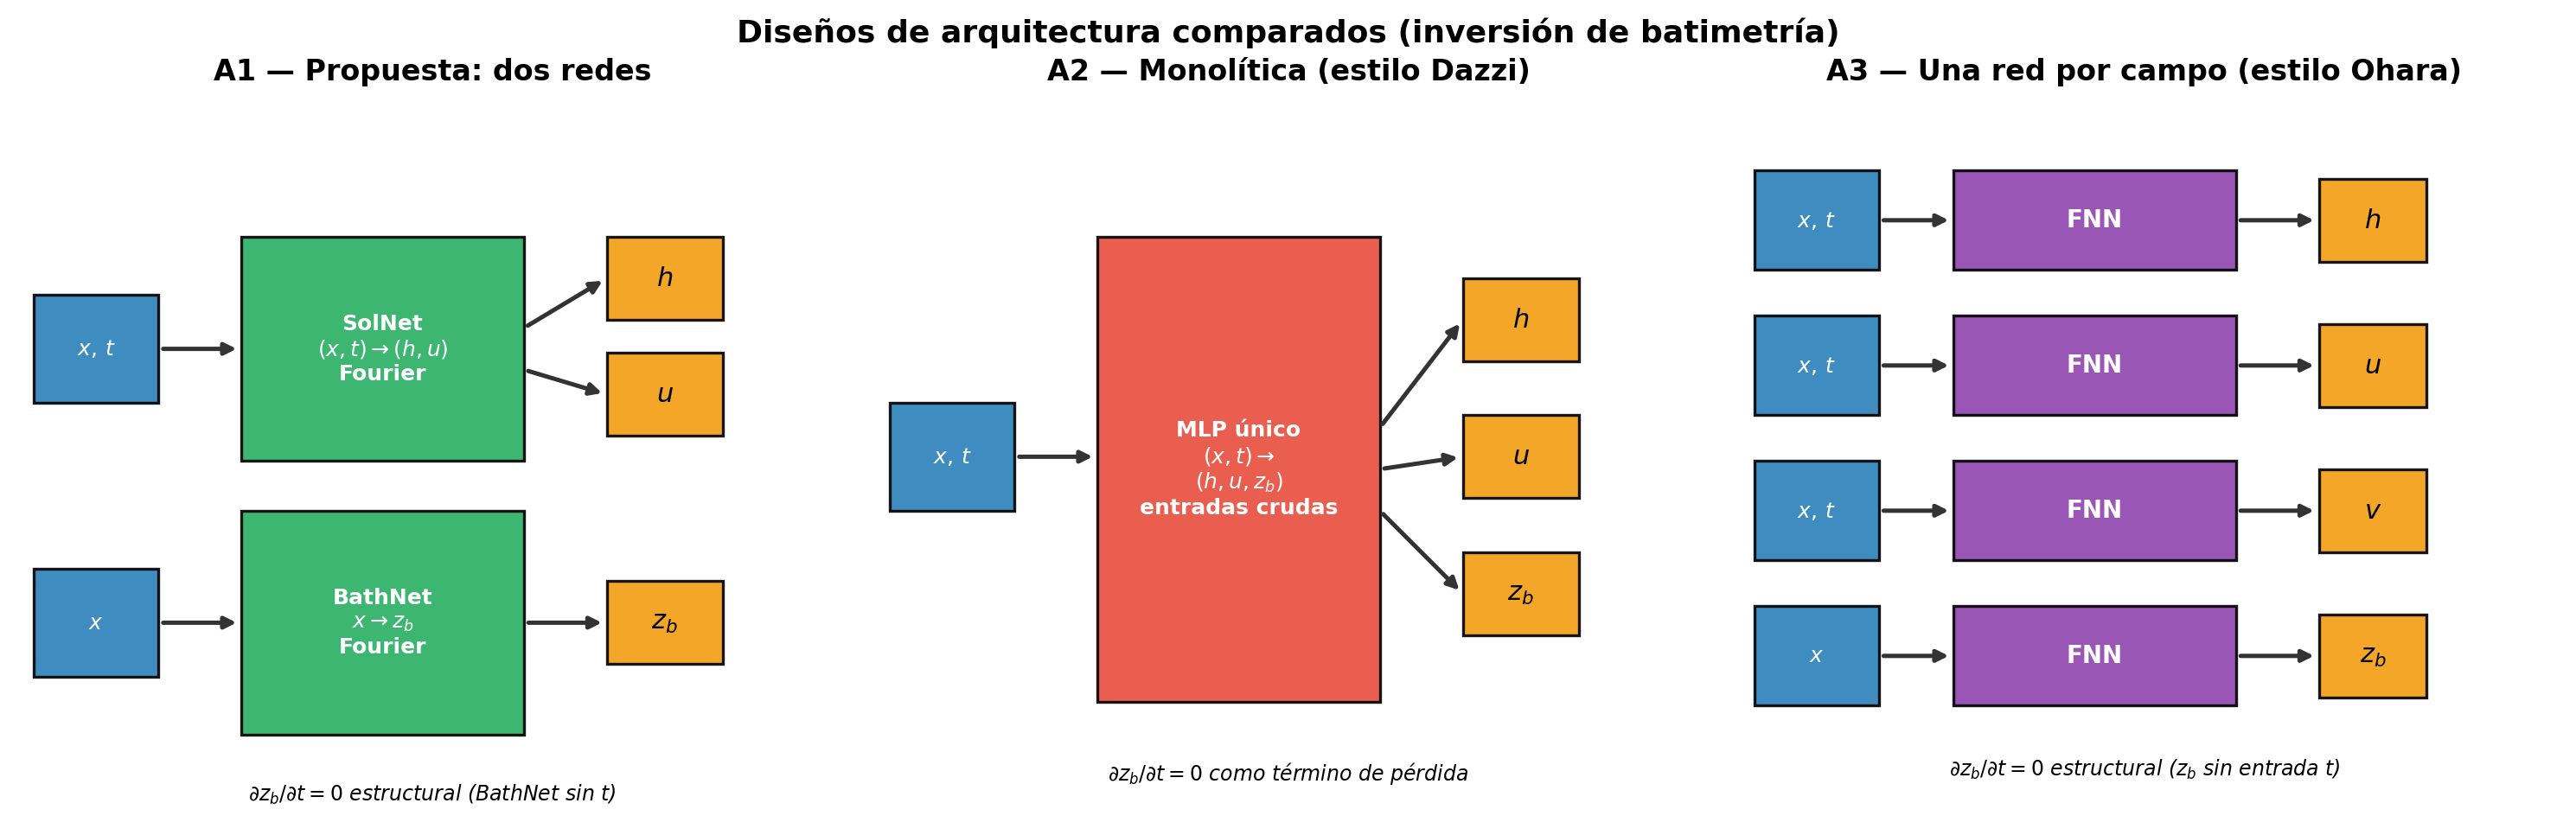
\includegraphics[width=\textwidth]{figures/architecture_designs.png}
  \caption{Los tres diseños de arquitectura comparados, todos para el problema
           inverso de batimetría. \textbf{A1} (propuesta): dos redes ---
           SolNet y BathNet ---, con BathNet sin entrada $t$
           ($\partial\zb/\partial t = 0$ estructural) y embedding de Fourier.
           \textbf{A2} (estilo Dazzi): una red monolítica que produce
           $(h,u,\zb)$ conjuntamente, con $\partial\zb/\partial t = 0$
           impuesto como término de pérdida. \textbf{A3} (estilo Ohara): una
           red totalmente conectada por cada campo de salida. Cada diseño se
           evalúa en el estudio de escalamiento a presupuestos de
           $\approx$20K, 100K y 500K parámetros.}
  \label{fig:arch}
\end{figure}

\subsection{Caso base}

Las ecuaciones de aguas someras, sus hipótesis de validez y la notación se
introdujeron en la Sección~\ref{sec:problema}. El caso base de este trabajo
(Exp.~1) las especializa a flujo 1D estacionario sin fricción:
%
\begin{align}
  \text{Continuidad:} \quad & \pd{(hu)}{x} = 0 \label{eq:cont} \\
  \text{Momento:}     \quad & u\pd{u}{x} + g\pd{(h + \zb)}{x} = 0 \label{eq:mom}
\end{align}

\subsection{Formas del residuo}

La Sección~\ref{sec:problema} señaló que las SWE admiten formas equivalentes;
su elección es una decisión metodológica y un aporte de este trabajo, evaluado
en la Sección~\ref{sec:ablation}. Se comparan tres formulaciones del residuo,
concretadas para el caso base:

\paragraph{Forma primitiva.}
Residuos directos de \eqref{eq:cont}--\eqref{eq:mom}:
\begin{align}
  r_{\text{cont}} &= u\,\pd{h}{x} + h\,\pd{u}{x}, \label{eq:r-prim-cont}\\
  r_{\text{mom}}  &= u\,\pd{u}{x} + g\Big(\pd{h}{x} + \pd{\zb}{x}\Big).
    \label{eq:r-prim-mom}
\end{align}

\paragraph{Forma primitiva-conservativa.}
Ponderación mediante la matriz $\bm{A}$:
\begin{equation}
  \begin{pmatrix} R_{\text{cont}} \\ R_{\text{mom}} \end{pmatrix}
  = \underbrace{\begin{pmatrix} 1 & 0 \\ u & h \end{pmatrix}}_{\bm{A}}
  \begin{pmatrix} r_{\text{cont}} \\ r_{\text{mom}} \end{pmatrix}
  \label{eq:primcons}
\end{equation}

\paragraph{Forma conservativa.}
Residuos sobre flujos conservativos:
\begin{align}
  R_{\text{masa}} &= \pd{(hu)}{x}, \label{eq:r-cons-masa}\\
  R_{\text{mom}}  &= \pd{}{x}\!\Big(hu^2 + \tfrac{1}{2}gh^2\Big)
                     + gh\,\pd{\zb}{x}. \label{eq:r-cons-mom}
\end{align}

\subsection{Función de pérdida}

\begin{equation}
  \mathcal{L} = \lambda_{\eta}\mathcal{L}_{\eta}
              + \lambda_{\text{PDE}}\mathcal{L}_{\text{PDE}}
              + \lambda_q \mathcal{L}_q
              + \lambda_{\text{BC}}\mathcal{L}_{\text{BC}}
              + \lambda_{\text{TV}}\mathcal{L}_{\text{TV}}
              + \lambda_{\text{Tikh}}\mathcal{L}_{\text{Tikh}}
              + \lambda_{\text{pos}}\mathcal{L}_{\text{pos}}
  \label{eq:loss}
\end{equation}

con (todas las sumas son promedios sobre los puntos correspondientes):
\begin{align*}
  \mathcal{L}_{\eta}       &= \tfrac{1}{|S|}\sum_{i\in S}
                              \big(h_i + z_{b,i} - \eta^{\text{obs}}_i\big)^2, \\
  \mathcal{L}_{\text{PDE}}  &= \tfrac{1}{N_c}\sum_i
                              \big(R_{\text{cont},i}^2 + R_{\text{mom},i}^2\big), \\
  \mathcal{L}_q            &= \tfrac{1}{N}\sum_i (h_i u_i - q)^2, \\
  \mathcal{L}_{\text{BC}}   &= \zb(x_L)^2 + \zb(x_R)^2
                              + \big(h(x_R)-h_{\text{down}}\big)^2, \\
  \mathcal{L}_{\text{TV}}   &= \tfrac{1}{N-1}\sum_i |z_{b,i+1}-z_{b,i}|/\Delta x, \\
  \mathcal{L}_{\text{Tikh}} &= \tfrac{1}{N}\sum_i z_{b,i}^2, \\
  \mathcal{L}_{\text{pos}}  &= \tfrac{1}{N}\sum_i \max(0,-h_i)^2 .
\end{align*}
$\mathcal{L}_\eta$ es la pérdida de datos sobre la superficie libre, evaluada
solo en el subconjunto observado $S$ (admite observaciones dispersas);
$\mathcal{L}_{\text{PDE}}$ el residuo físico de la forma elegida;
$\mathcal{L}_q$ fija el caudal por unidad de ancho conocido $q = hu$;
$\mathcal{L}_{\text{BC}}$ impone fondo nulo en los extremos y la profundidad
prescrita aguas abajo; $\mathcal{L}_{\text{TV}}$ y $\mathcal{L}_{\text{Tikh}}$
regularizan $\zb$ (variación total y Tikhonov); y $\mathcal{L}_{\text{pos}}$
penaliza profundidades negativas. Cuando hay observaciones de velocidad se
añade un término análogo $\mathcal{L}_u = \tfrac{1}{|S|}\sum_{i\in S}
(u_i-u^{\text{obs}}_i)^2$ (peso $\lambda_u$); el Exp.~1 lo explota para
cuantificar el aporte de la velocidad. La Tabla~\ref{tab:pesos} lista los
pesos del caso base. Esta misma función de pérdida, con los mismos pesos, se
emplea para las tres arquitecturas evaluadas (Sección~\ref{sec:protocolo}), de
modo que la comparación aísla el efecto de la arquitectura.

\begin{table}[H]
\centering
\caption{Pesos de pérdida del caso base (Exp.~1).}
\label{tab:pesos}
\begin{tabular}{lc}
\toprule
Término & Peso \\
\midrule
$\lambda_{\eta}$ (datos $\eta$)         & 10 \\
$\lambda_{u}$ (datos $u$, opcional)     & 1 \\
$\lambda_{\text{PDE}}$ (residuo SWE)    & 1 \\
$\lambda_{q}$ (caudal)                  & 10 \\
$\lambda_{\text{BC}}$ (bordes)          & 100 \\
$\lambda_{\text{TV}}$ (variación total) & $10^{-4}$ \\
$\lambda_{\text{Tikh}}$ (Tikhonov)      & $10^{-5}$ \\
$\lambda_{\text{pos}}$ (positividad)    & 10 \\
\bottomrule
\end{tabular}
\end{table}

\subsection{Métricas de evaluación}

La calidad de la batimetría recuperada se cuantifica con:
\begin{align*}
  \RMSE  &= \sqrt{\tfrac{1}{N}\sum_i (\hat z_{b,i}-z_{b,i})^2}, \qquad
  \NRMSE  = \frac{\RMSE}{\max_i z_{b,i} - \min_i z_{b,i}}, \\
  R^2    &= 1 - \frac{\sum_i (\hat z_{b,i}-z_{b,i})^2}
                     {\sum_i (z_{b,i}-\bar z_b)^2}.
\end{align*}
El $\NRMSE$ normaliza por el rango de $\zb$ (convención de Angel et al.\, para
comparar con su $\approx$14--16\,\%); $R^2$ mide la fracción de varianza
explicada.

\subsection{Entrenamiento}

Dos fases: 12K épocas de Adam (lr $= 10^{-3}$, decay $\times 0.5$ cada 2K)
seguidas de 600 pasos de L-BFGS con line search de Wolfe. La segunda fase
proporciona convergencia de segundo orden para el refinamiento final. En el
caso base 1D, el residuo físico se evalúa sobre la malla espacial completa
(puntos de colocación); las observaciones pueden ser un subconjunto disperso
$S$ de esa malla, lo que conecta con el estudio de densidad de observaciones
del Exp.~1 (Sección~\ref{sec:exp}).

\subsection{Protocolo de comparación justa}
\label{sec:protocolo}

Para que las diferencias observadas sean atribuibles al diseño de la
arquitectura y no a factores de confusión, los tres diseños de la
Sección~\ref{sec:arquitecturas} se entrenan bajo un protocolo idéntico:

\begin{itemize}
  \item \textbf{Mismo presupuesto de parámetros.} En cada punto de comparación
        los tres diseños se instancian al mismo presupuesto (pequeño, medio o
        grande); el número de parámetros es el eje que se barre, no una
        variable libre.
  \item \textbf{Mismos datos.} El mismo ground truth y las mismas
        observaciones ($\eta$, o $\eta$ y $u$) en cada caso de prueba.
  \item \textbf{Misma pérdida.} La función de pérdida
        (Ecuación~\ref{eq:loss}), con los mismos pesos.
  \item \textbf{Misma forma del residuo.} La forma primitiva; la ablación de
        la Sección~\ref{sec:ablation} evalúa cuál de las tres formas resulta
        más adecuada.
  \item \textbf{Mismo presupuesto de entrenamiento.} 12K épocas de Adam $+$
        600 pasos de L-BFGS.
  \item \textbf{Mismas semillas.} Tres semillas aleatorias por configuración;
        se reporta media $\pm$ desviación estándar.
  \item \textbf{Mismo hardware.} GPU NVIDIA RTX 4090.
\end{itemize}

\paragraph{Métricas de costo.}
Junto con la precisión ($\RMSE$, $\NRMSE$ y $R^2$ de $\zb$), se reporta el
\emph{costo} de cada configuración:
\begin{itemize}
  \item \textbf{Parámetros entrenables}: el costo de capacidad; es el eje que
        se barre en el estudio de escalamiento (presupuestos pequeño, medio y
        grande).
  \item \textbf{Tiempo de entrenamiento} (wall-time) bajo el presupuesto de
        entrenamiento fijo.
  \item \textbf{Memoria de GPU} (VRAM pico).
\end{itemize}
La comparación contrasta precisión frente a costo: a presupuesto de parámetros
igualado, qué diseño es más preciso; y, a lo largo del barrido, qué diseño
domina la curva precisión-vs-parámetros. El estudio se ejecuta sobre los casos
de prueba Exp.~1, 2 y 3 (Sección~\ref{sec:exp}); sus resultados se reportan en
la Sección~\ref{sec:arch-comp}.

\section{Experimentos}
\label{sec:exp}

Este capítulo presenta la evaluación experimental en tres bloques: la
comparación controlada de las tres arquitecturas
(Sección~\ref{sec:arch-comp}); seis casos de prueba de complejidad creciente
---del régimen 1D estacionario a datos reales de laboratorio--- que conforman
el banco de pruebas (Secciones~\ref{sec:exp1} a~\ref{sec:exp6}); y la ablación
de la forma del residuo SWE (Sección~\ref{sec:ablation}). Cada caso se
especifica a continuación; sus resultados se completarán con las corridas del
estudio comparativo de arquitecturas.

\subsection{Comparación de arquitecturas}
\label{sec:arch-comp}

Este estudio compara los tres diseños de arquitectura de la
Sección~\ref{sec:arquitecturas} --- la propuesta de dos redes (A1), la
monolítica estilo Dazzi (A2) y la de una red por campo estilo Ohara (A3) ---
mediante un
\emph{estudio de escalamiento}: cada diseño se instancia a tres presupuestos
de parámetros (pequeño $\approx$20K, medio $\approx$100K, grande
$\approx$500K) y se evalúa en tres casos de complejidad creciente --- el bump
subcrítico 1D estacionario (Exp.~1), la cuenca de Thacker 1D transitoria
(Exp.~2) y los dos cilindros 2D (Exp.~3) ---, bajo el protocolo de comparación
justa de la Sección~\ref{sec:protocolo}. El resultado es doble: (i) a
presupuesto de parámetros igualado, qué diseño recupera mejor la batimetría
--- comparación que aísla el diseño de la capacidad ---; y (ii) la curva de
precisión ($\RMSE$, $\NRMSE$, $R^2$ de $\zb$) frente al número de parámetros
de cada diseño, que sitúa a la propuesta en la frontera precisión-costo. Se
reporta además el costo de cómputo (tiempo de entrenamiento y VRAM pico). Los
tres diseños se ordenan por su \emph{grado de separación de redes}: monolítica
(A2), flujo agrupado con batimetría aparte (A1) y una red por cada campo (A3).
El objetivo es ubicar a la propuesta en ese eje --- si darle red propia a
$\zb$ y agrupar el flujo con embedding de Fourier le da ventaja sobre la red
monolítica y sobre la separación total por campo, y en qué rango de
presupuestos.

\paragraph{Resultados.}
\pendiente{tabla del estudio de escalamiento (3 diseños $\times$ 3 presupuestos
$\times$ 3 casos) y figura de la frontera precisión--parámetros.}

% ──────────────────────────────────────────────────────────────
\subsection{Exp.\ 1 --- Bump subcrítico 1D (estacionario)}
\label{sec:exp1}

\paragraph{Setup.}
Bump parabólico de 200\,mm en dominio $[-10, 10]$\,m, descarga
$q = 4.42$\,m$^2$/s, profundidad aguas abajo $h_{\text{down}} = 2.0$\,m,
sin fricción. Rango de Froude: $[0.50, 0.63]$. Depresión superficial:
93\,mm. El planteamiento y la solución analítica (ecuación de Bernoulli) se
detallan en el Apéndice~\ref{app:exp1}.

\paragraph{Resultados.}
\pendiente{resultados del estudio de arquitecturas.}

% ──────────────────────────────────────────────────────────────
\subsection{Exp.\ 2 --- Cuenca de Thacker 1D (transitorio)}
\label{sec:exp2}

\paragraph{Setup.}
Cuenca parabólica $\zb = 0.5(x^2 - 1)$ en $[-2, 2]$\,m, profundidad
central $h_0 = 0.5$\,m, período de oscilación $T = 2.006$\,s.
Problema cerrado sin condiciones de borde de flujo. El planteamiento y la
solución analítica de Thacker se detallan en el Apéndice~\ref{app:exp2}.

\paragraph{Resultados.}
\pendiente{resultados del estudio de arquitecturas.}

% ──────────────────────────────────────────────────────────────
\subsection{Exp.\ 3 --- Dos cilindros 2D (transitorio)}
\label{sec:exp3}

\paragraph{Setup.}
Dos obstáculos cilíndricos en un dominio 2D; observaciones $\eta$, $u$ y $v$
sobre una malla $40\times40$ y 15 instantáneas temporales. El planteamiento y
la solución de referencia numérica se detallan en el Apéndice~\ref{app:exp3}.

\paragraph{Resultados.}
\pendiente{resultados del estudio de arquitecturas.}

% ──────────────────────────────────────────────────────────────
\subsection{Exp.\ 4 --- Topografía variable 2D (Tian dT10)}
\label{sec:exp4}

\paragraph{Setup.}
Réplica fiel del caso dinámico \emph{dT10} de Tian et al.\ \cite{tian2025}
(Sección~3.3): masa de agua sobre topografía oscilatoria 2D que parte de un
estado desbalanceado ($h(x,y,0) = \zb$) y se relaja bajo gravedad con bordes
periódicos, sin forzamiento externo. El planteamiento y la solución de
referencia numérica se detallan en el Apéndice~\ref{app:exp4}.

\paragraph{Resultados.}
\pendiente{resultados del estudio de arquitecturas.}

% ──────────────────────────────────────────────────────────────
\subsection{Exp.\ 5 --- Cuenca cerrada (paraboloide de Thacker)}
\label{sec:exp5}

\paragraph{Setup.}
Cuenca cuyo borde emerge sobre el nivel medio (75.5\% del dominio siempre
seco) y \emph{sin} forzamiento de borde externo. El planteamiento y la
solución analítica de Thacker 2D se detallan en el Apéndice~\ref{app:exp5}.

\paragraph{Resultados.}
\pendiente{resultados del estudio de arquitecturas.}

% ──────────────────────────────────────────────────────────────
\subsection{Exp.\ 6 --- Datos reales (canal de oleaje de Angel)}
\label{sec:exp6}

\paragraph{Setup.}
Datos \emph{reales} del canal de Hamburgo de Angel et al.\ \cite{angel2024},
ventana de oleaje establecido $t\in[40,60]$\,s; el sensor S1 ($x=1.5$\,m)
impone la entrada como Dirichlet \emph{soft} (penalización MSE con el
mismo peso que la observación interior, no es una BC dura --- el método
adjoint de Angel sí impone la BC dura a través del solver directo, lo
que parcialmente explica el cierre del gap NRMSE) y S2 ($x=3.5$\,m),
fuera del bump, es la observación interior; PINN transitorio 1D con
drag de fondo lineal y $\zb\ge0$.

\paragraph{Resultados.}
\pendiente{resultados del estudio de arquitecturas.}

% ──────────────────────────────────────────────────────────────
\subsection{Estudio de ablación: forma de ecuación SWE}
\label{sec:ablation}

Se comparan las tres formas del residuo SWE (Sección~\ref{sec:method})
en el caso del bump subcrítico (Exp.\ 1), con la misma arquitectura,
pesos de pérdida y presupuesto de entrenamiento. Cada forma se entrena
con semillas aleatorias independientes para evaluar la robustez.

\paragraph{Resultados.}
\pendiente{tabla comparativa de las tres formas del residuo (RMSE, $R^2$ y
robustez entre semillas).}

\section{Comparación con la Literatura}
\label{sec:comp}

\subsection{Tesis vs.\ Dazzi et al.\ (2024)}

Ambos trabajan sobre el mismo ground truth (bump B1 y Thacker T1), lo que
permite comparación directa de arquitectura, aunque los \emph{problemas}
difieren: Dazzi resuelve el problema directo mientras que esta tesis
resuelve el inverso.

\begin{table}[H]
\centering
\caption{Comparación arquitectónica: Dazzi et al.\ (2024) vs.\ esta tesis.}
\label{tab:dazzi-comp}
\begin{tabular}{lll}
\toprule
Característica & Dazzi et al.\ (2024) & Esta tesis \\
\midrule
Tarea & Directa (aprender $h, u, \zb$) & Inversa (recuperar $\zb$) \\
Red & MLP único $\to (h, u, \zb)$ & SolNet + BathNet \\
Parámetros & 543{,}603 & 17{,}923 \\
Forma SWE & Aumentada (4 ecs.) & Primitiva (2 ecs.) \\
$\zb$ temporal & $\partial \zb/\partial t = 0$ como loss & Estructural (sin $t$) \\
Encoding & Raw $(x,t)$ & Fourier features \\
Entrenamiento & Adam (30K) & Adam (12K) + L-BFGS (600) \\
\bottomrule
\end{tabular}
\end{table}

La propuesta (A1) usa cerca de \textbf{30$\times$ menos parámetros} que Dazzi
(17\,923 frente a 543\,603), apoyándose en tres elementos de diseño: (1) el
embedding de Fourier, que compensa la red más pequeña; (2) la imposición
estructural de $\partial \zb / \partial t = 0$, que elimina un hiperparámetro;
y (3) el refinamiento con L-BFGS. Si esa reducción de capacidad mantiene una
precisión comparable es lo que cuantifica el estudio de escalamiento de la
Sección~\ref{sec:arch-comp}. \pendiente{comparación de precisión frente a
Dazzi sobre el bump B1.}

\subsection{Tesis vs.\ Angel et al.\ (2024)}

Angel et al.\ establecen el primer benchmark de inversión de batimetría
con datos experimentales reales; su método adjunto-SWE alcanza un NRMSE de
$\approx$14--16\,\% con 2 sensores.

\begin{table}[H]
\centering
\caption{Comparación de enfoque: Angel et al.\ (2024) vs.\ esta tesis.}
\label{tab:angel-comp}
\begin{tabular}{lll}
\toprule
Propiedad & Angel et al.\ (2024) & Esta tesis \\
\midrule
Método & Adjunto + desc.\ gradiente & PINN \\
Modelo & SWE 1D (Dedalus, $M=68$) & SWE 1D (AD sobre redes) \\
Datos & Reales (canal de oleaje) & Reales (Exp.\ 6) + sintéticos \\
Observaciones & 3 sensores puntuales & Grilla / sensores dispersos \\
Bump & Gaussiano, 200\,mm & Parabólico, 200\,mm \\
$kh$ & 1.3 (intermedio) & $\ll 1$ (SWE exacto) \\
\bottomrule
\end{tabular}
\end{table}

\paragraph{Exp.\ 6 --- comparación con Angel.}
El Exp.~6 (Sección~\ref{sec:exp6}) aplica el PINN propuesto a estos mismos
datos reales; el contraste con el método de restricción \textbf{dura} de
Angel (NRMSE $\approx$14--16\,\%) es el núcleo de la comparación. El método
adjunto impone la SWE como restricción dura mediante un solver directo,
mientras que el PINN de penalización \textbf{blanda} admite la equifinalidad
$\eta = h + \zb$ cuando los sensores están fuera del bump.
\pendiente{recuperación cuantitativa del PINN sobre los datos de Angel y el
diagnóstico blando-vs-duro.}

\subsection{Hallazgo sobre formas de ecuación}

El estudio de ablación (Sección~\ref{sec:ablation}) constituye una
\textbf{contribución original}: ningún trabajo previo compara formas
del residuo SWE específicamente para el problema \emph{inverso}.
Tian et al.\ \cite{tian2025} demuestran la ventaja de la forma
primitiva-conservativa para el problema directo; la ablación de esta tesis
determina qué forma es preferible para la inversión. \pendiente{resultado de
la ablación de formas del residuo.}

\section{Conclusiones y Trabajo Futuro}
\label{sec:concl}

\subsection{Contribuciones}

\begin{enumerate}
  \item \textbf{Arquitectura eficiente}: se propone una arquitectura de dos
        redes ($\approx$18K parámetros) con Fourier features e imposición
        estructural de $\partial \zb/\partial t = 0$, frente a los
        $\approx$544K de la arquitectura monolítica de Dazzi.
        \pendiente{cuantificación de su precisión frente a A2 y A3 en el
        estudio de escalamiento (Sección~\ref{sec:arch-comp}).}

  \item \textbf{Equifinalidad}: se caracterizan cuatro mecanismos para romper
        la degeneración $(h, \zb)$ del problema inverso ---observaciones de
        velocidad, muestreo temporal, condiciones de borde y la pérdida
        $\mathcal{L}_{\zb,\text{IC}}$---; su eficacia se evalúa en los casos
        de prueba (Sección~\ref{sec:exp}).

  \item \textbf{Formas de ecuación para inversión}: primer estudio comparativo
        de las formas primitiva, primitiva-conservativa y conservativa del
        residuo SWE en el problema inverso (Sección~\ref{sec:ablation}).
        \pendiente{conclusión sobre qué forma del residuo es más robusta para
        la inversión.}

  \item \textbf{Robustez}: el banco de pruebas evalúa la tolerancia del método
        al ruido en las observaciones y a la densidad de muestreo.
        \pendiente{niveles de ruido y densidad de observaciones tolerados.}

  \item \textbf{Límite con datos reales (Exp.\ 6)}: se evalúa de forma
        reproducible si el PINN de penalización blanda recupera la batimetría
        de los datos reales de Angel et al., frente al método adjunto de
        restricción dura. La barrera potencial es estructural ---la
        equifinalidad $\eta = h + \zb$ bajo física blanda con sensores fuera
        del bump---, no computacional.
        \pendiente{recuperación del PINN sobre los datos de Angel y
        comparación con el benchmark adjunto.}
\end{enumerate}

\subsection{Trabajo futuro}

\begin{itemize}
  \item \textbf{Restricción dura de la EDP}: motivado por la dificultad del
        PINN de penalización blanda sobre datos reales (Exp.\ 6), integrar un
        solver directo SWE diferenciable en el lazo (híbrido PINN--adjunto),
        entrenamiento causal/curriculum, o ponderación adaptativa de residuos,
        para cerrar la brecha con el benchmark adjunto de Angel sobre datos
        reales.
  \item \textbf{Formas de ecuación}: extender la comparación de formas del
        residuo al caso transitorio 2D con wetting-drying.
  \item \textbf{Co-inversión de fricción}: aprender simultáneamente $\zb$
        y el coeficiente de Manning $n$.
  \item \textbf{Escalabilidad}: evaluar factibilidad en dominios 2D reales
        (río Sacramento, $\sim$10K puntos).
\end{itemize}


% ── Apéndices ──
\appendix
\section{Casos sintéticos: planteamiento y soluciones de referencia}
\label{app:casos-sinteticos}

Este apéndice especifica, para cada caso de prueba con datos sintéticos
(Exp.~1 a~5), el planteamiento matemático del problema --- ecuaciones de
gobierno, dominio, condiciones de borde e iniciales y batimetría --- y su
solución de referencia. Para los casos con solución analítica cerrada
(Exp.~1, 2 y 5) se da la expresión exacta; para los casos sin forma cerrada
(Exp.~3 y 4) la referencia es la solución numérica de un esquema de volúmenes
finitos. Las ecuaciones de aguas someras (SWE) y su notación se introdujeron
en la Sección~\ref{sec:problema}; aquí se particularizan a cada caso. La
gravedad es $g = 9.81$\,m\,s$^{-2}$.

\subsection{Exp.\ 1 --- Bump subcrítico 1D}
\label{app:exp1}

\paragraph{Problema.}
Flujo 1D estacionario sin fricción sobre un bump parabólico, gobernado por las
SWE estacionarias (caudal específico $q = h u$ constante y conservación de la
energía). La batimetría es
\begin{equation}
  \zb(x) =
  \begin{cases}
    H_b - \dfrac{H_b}{w^2}\,(x - x_0)^2, & |x - x_0| < w,\\[1.2ex]
    0, & \text{en otro caso,}
  \end{cases}
\end{equation}
con altura $H_b = 0.2$\,m, semiancho $w = 2$\,m y centro $x_0 = 0$, en el
dominio $[-10, 10]$\,m. Las condiciones de borde son el caudal específico
$q = 4.42$\,m$^2$/s aguas arriba y la profundidad $h_{\text{down}} = 2.0$\,m
aguas abajo.

\paragraph{Solución de referencia (analítica).}
En flujo estacionario sin fricción la energía específica se conserva a lo
largo del canal (ecuación de Bernoulli):
\begin{equation}
  \frac{q^2}{2 g\,h(x)^2} + h(x) + \zb(x) = C,
  \label{eq:app-bernoulli}
\end{equation}
donde la constante $C$ se fija con la condición aguas abajo,
$C = q^2/(2 g\,h_{\text{down}}^2) + h_{\text{down}} + \zb(x_{\text{fin}})$.
Multiplicando \eqref{eq:app-bernoulli} por $h^2$ se obtiene, en cada $x$, la
ecuación cúbica
\begin{equation}
  h^3 + \bigl(\zb(x) - C\bigr)\,h^2 + \frac{q^2}{2 g} = 0,
\end{equation}
de cuyas raíces se toma la \emph{subcrítica}: real, positiva y mayor que la
profundidad crítica $h_c = (q^2/g)^{1/3}$. La velocidad y la superficie libre
son $u(x) = q/h(x)$ y $\eta(x) = h(x) + \zb(x)$. El planteamiento sigue a
Delestre et al.\ \cite{delestre2013} (compilación SWASHES) y a Dazzi et al.\
\cite{dazzi2024}.

\subsection{Exp.\ 2 --- Cuenca de Thacker 1D}
\label{app:exp2}

\paragraph{Problema.}
Oscilación no lineal de una masa de agua en una cuenca parabólica cerrada,
gobernada por las SWE 1D transitorias sin fricción. La batimetría es
\begin{equation}
  \zb(x) = h_0\left(\frac{x^2}{a^2} - 1\right),
\end{equation}
con profundidad característica $h_0 = 0.5$\,m y semiancho $a = 1$\,m, en el
dominio $[-2, 2]$\,m. El problema es cerrado: no hay condiciones de borde de
flujo, y la condición inicial es la solución analítica evaluada en $t = 0$.

\paragraph{Solución de referencia (analítica).}
Thacker \cite{thacker1981} obtuvo una solución exacta de superficie libre
plana con línea de costa móvil. La frecuencia angular y el período de
oscilación son
\begin{equation}
  \omega = \frac{\sqrt{2 g h_0}}{a},
  \qquad T = \frac{2\pi}{\omega} \approx 2.006~\text{s},
\end{equation}
y los campos
\begin{align}
  h(x,t)    &= \max\!\left(0,\;
               h_0\left[1 - \left(\frac{x + \tfrac{1}{2}\cos(\omega t)}{a}\right)^{\!2}\,\right]\right),\\
  u(x,t)    &= \tfrac{1}{2}\,\omega\,\sin(\omega t)
               \quad\text{donde } h > 0\ \ (\text{0 en seco}),\\
  \eta(x,t) &= h(x,t) + \zb(x).
\end{align}
La superficie libre permanece plana y oscila en el tiempo, mientras la línea
de costa se desplaza. El caso está también compilado en SWASHES
\cite{delestre2013}.

\subsection{Exp.\ 3 --- Dos cilindros 2D}
\label{app:exp3}

\paragraph{Problema.}
Flujo 2D transitorio sobre dos obstáculos cilíndricos sólidos, gobernado por
las SWE 2D en forma conservativa,
$\bm{U}_t + \bm{F}(\bm{U})_x + \bm{G}(\bm{U})_y = \bm{S}(\bm{U}, \zb)$ con
$\bm{U} = (h, hu, hv)$. La configuración se replica fielmente del benchmark
2D de Ruppenthal y Kuzmin \cite{ruppenthal2026} (Sección~7.2). La batimetría
consiste en dos cilindros con paredes verticales (sin suavizado),
\begin{equation}
  \zb(x,y) =
  \begin{cases}
    0.2\,\text{m}, & \text{si } \sqrt{(x-8)^2 + (y-8)^2} \le 4\,\text{m}, \\
    0.3\,\text{m}, & \text{si } \sqrt{(x-15)^2 + (y-15)^2} \le 2\,\text{m}, \\
    0,             & \text{en otro caso,}
  \end{cases}
\end{equation}
en el dominio $[0, 25]^2$\,m. Los dos cilindros (alturas $H_1 = 0.2$ y
$H_2 = 0.3$\,m, radios $R_1 = 4$ y $R_2 = 2$\,m) están alineados sobre la
diagonal $x = y$, paralelos a la dirección del flujo inicial. La condición
inicial corresponde a superficie libre en reposo y velocidad uniforme:
\begin{equation}
  \eta(x,y,0) = h + \zb = 2\,\text{m}, \qquad
  \bm{v}(x,y,0) = (2.21,\ 2.21)\,\text{m/s},
\end{equation}
de modo que la profundidad inicial $h(x,y,0) = 2 - \zb(x,y)$ es menor sobre
los cilindros que sobre el lecho plano. Tiempo final $T = 60$\,s con paso
$\Delta t = 10^{-2}$\,s.

\paragraph{Solución de referencia (numérica).}
Este caso no admite solución analítica cerrada. La referencia se obtiene
resolviendo las SWE 2D sobre una malla cartesiana de $50\times 50$ celdas
($\Delta x = \Delta y = 0.5$\,m), con un esquema de volúmenes finitos, flujos
numéricos de tipo HLL (Harten--Lax--van~Leer) sobre estados reconstruidos
por la técnica hidrostática de Audusse \cite{audusse2004}, well-balanced
para topografía discontinua; el término fuente topográfico queda absorbido
en correcciones de presión en las interfaces, siguiendo en lo demás la
formulación estándar de LeVeque \cite{leveque2002}. Las condiciones de
frontera son Dirichlet de inflow en las dos caras por las que entra el
flujo --$x = 0$ y $y = 0$-- prescribiendo el estado uniforme
$(h, u, v) = (\eta_0, u_0, v_0)$ vía celdas fantasma; las caras opuestas
($x = L_x$, $y = L_y$) usan extrapolación de gradiente cero (outflow).
Ruppenthal y Kuzmin no especifican BCs explícitamente para §7.2; ésta
es la elección más natural para preservar la corriente uniforme
prescrita en la CI a lo largo de los 60\,s simulados. Ruppenthal y Kuzmin emplean un esquema de
elementos finitos con limiters de flujo (MCL) sobre la misma malla; ambas
son discretizaciones estándar y convergentes de las SWE.

\subsection{Exp.\ 4 --- Topografía variable 2D (Tian dT10)}
\label{app:exp4}

\paragraph{Problema.}
Flujo 2D transitorio sobre una topografía oscilatoria, gobernado por las SWE
2D en forma conservativa. La configuración se replica fielmente del caso
dinámico \emph{dT10} de Tian et al.\ \cite{tian2025} (Sección~3.3),
denominado allí ``problema mareal'' por analogía con la geometría de fondo
(no por la presencia de forzamiento mareal externo). La topografía es
\begin{equation}
  \zb(x,y) = 1 + 0{.}01\,\cos\!\left(\frac{\pi x}{2}\right)
                          \cos\!\left(\frac{\pi y}{2}\right),
\end{equation}
en el dominio $(x,y) \in [-2, 2]^2$\,m. Tiene máximos en el centro y en las
cuatro esquinas ($\zb = 1{.}01$\,m) y mínimos en los puntos medios de los
bordes ($\zb = 0{.}99$\,m). La condición inicial es desbalanceada respecto a
la superficie libre:
\begin{equation}
  h(x,y,0) = \zb(x,y), \qquad u(x,y,0) = v(x,y,0) = 0,
\end{equation}
de modo que la superficie libre inicial $\eta(x,y,0) = h + \zb = 2\zb$ hereda
el mismo patrón de máximos y mínimos. Bajo gravedad el agua fluye desde las
regiones altas (centro y esquinas) hacia las bajas (mitades de los bordes).
Las condiciones de borde son \emph{periódicas} en $x$ y $y$. Tiempo final
$T = 0{.}5$\,s.

\paragraph{Solución de referencia (numérica).}
Sin forma cerrada. Tian resuelve dT10 con el esquema entropy-stable ES1 de
Fjordholm et al.\ (2011) sobre una malla muy fina
($\Delta x = \Delta y = 0{.}01$\,m, CFL $= 0{.}25$). En esta tesis la
referencia se obtiene con el mismo solver FV-HLL del Exp.~3
(LeVeque \cite{leveque2002}) con condiciones de borde periódicas. Ambos
son esquemas estándar y convergentes para SWE con topografía variable.

\subsection{Exp.\ 5 --- Paraboloide de Thacker 2D}
\label{app:exp5}

\paragraph{Problema.}
Oscilación axisimétrica de una masa de agua en un paraboloide de revolución,
gobernada por las SWE 2D transitorias sin fricción. La batimetría es
\begin{equation}
  \zb(x,y) = -h_0\left(1 - \frac{r^2}{a^2}\right),
  \qquad r = \sqrt{(x - x_c)^2 + (y - y_c)^2},
\end{equation}
con $h_0 = 0.1$\,m, $a = 1$\,m y centro $(x_c, y_c) = (2, 2)$\,m, en el dominio
$[0, 4]^2$\,m. El problema es cerrado, con una frontera seco-mojado móvil.

\paragraph{Solución de referencia (analítica).}
Thacker \cite{thacker1981} obtuvo la solución exacta axisimétrica (compilada
en SWASHES \cite{delestre2013}). Con
\begin{equation}
  \omega = \frac{\sqrt{8 g h_0}}{a},
  \qquad
  A = \frac{a^2 - r_0^2}{a^2 + r_0^2},
\end{equation}
donde $r_0 = 0.8$\,m fija la amplitud de la oscilación, los campos son
\begin{align}
  h(x,y,t) &= h_0\left[
               \frac{\sqrt{1 - A^2}}{1 - A\cos(\omega t)} - 1
               - \frac{r^2}{a^2}\!
                 \left(\frac{1 - A^2}{(1 - A\cos(\omega t))^2} - 1\right)
              \right] - \zb(x,y),\\
  u(x,y,t) &= \frac{1}{2}\,
              \frac{\omega A \sin(\omega t)}{1 - A\cos(\omega t)}\,(x - x_c),\\
  v(x,y,t) &= \frac{1}{2}\,
              \frac{\omega A \sin(\omega t)}{1 - A\cos(\omega t)}\,(y - y_c),
\end{align}
con $h$ truncada a $0$ en la zona seca y $u = v = 0$ allí; la superficie libre
es $\eta = h + \zb$. La superficie permanece como un plano inclinado que
oscila en el tiempo.


% ── Bibliografía ──
\bibliographystyle{unsrtnat}
\bibliography{references}

\end{document}
